\documentclass[12pt]{article}


\usepackage{amssymb}
\usepackage{amsmath}
\usepackage{fullpage}
\usepackage{epsfig}
\usepackage{epstopdf, xcolor, hyperref}
\everymath{\displaystyle}



\begin{document}

\begin{center}
\underline{\LARGE{Volume by Slicing (Disks \& Washers)}}
\end{center}

\bigskip

\noindent SUGGESTED REFERENCE MATERIAL:

\bigskip

\noindent As you work through the problems listed below, you should reference Chapter 6.2 of the recommended textbook (or the equivalent chapter in your alternative textbook/online resource) and your lecture notes.

\bigskip

\noindent EXPECTED SKILLS:

\begin{itemize}

\item Be able to find the volume of a solid that consists of known cross-sectional areas. 

\item Know how to use the method of disks and washers to find the volume of a solid of revolution formed by revolving a region in the $xy$-plane about the $x-$axis, $y$-axis, or any other horizontal or vertical line.

\end{itemize}

\noindent PRACTICE PROBLEMS:

\medskip

\begin{enumerate}

\item For each of the following, set up but do not evaluate an integral (or integrals) which represent(s) the volume of the solid that results from revolving the shaded region around the indicated axis.

\begin{enumerate}

\item Around the $x$-axis:

\begin{center}

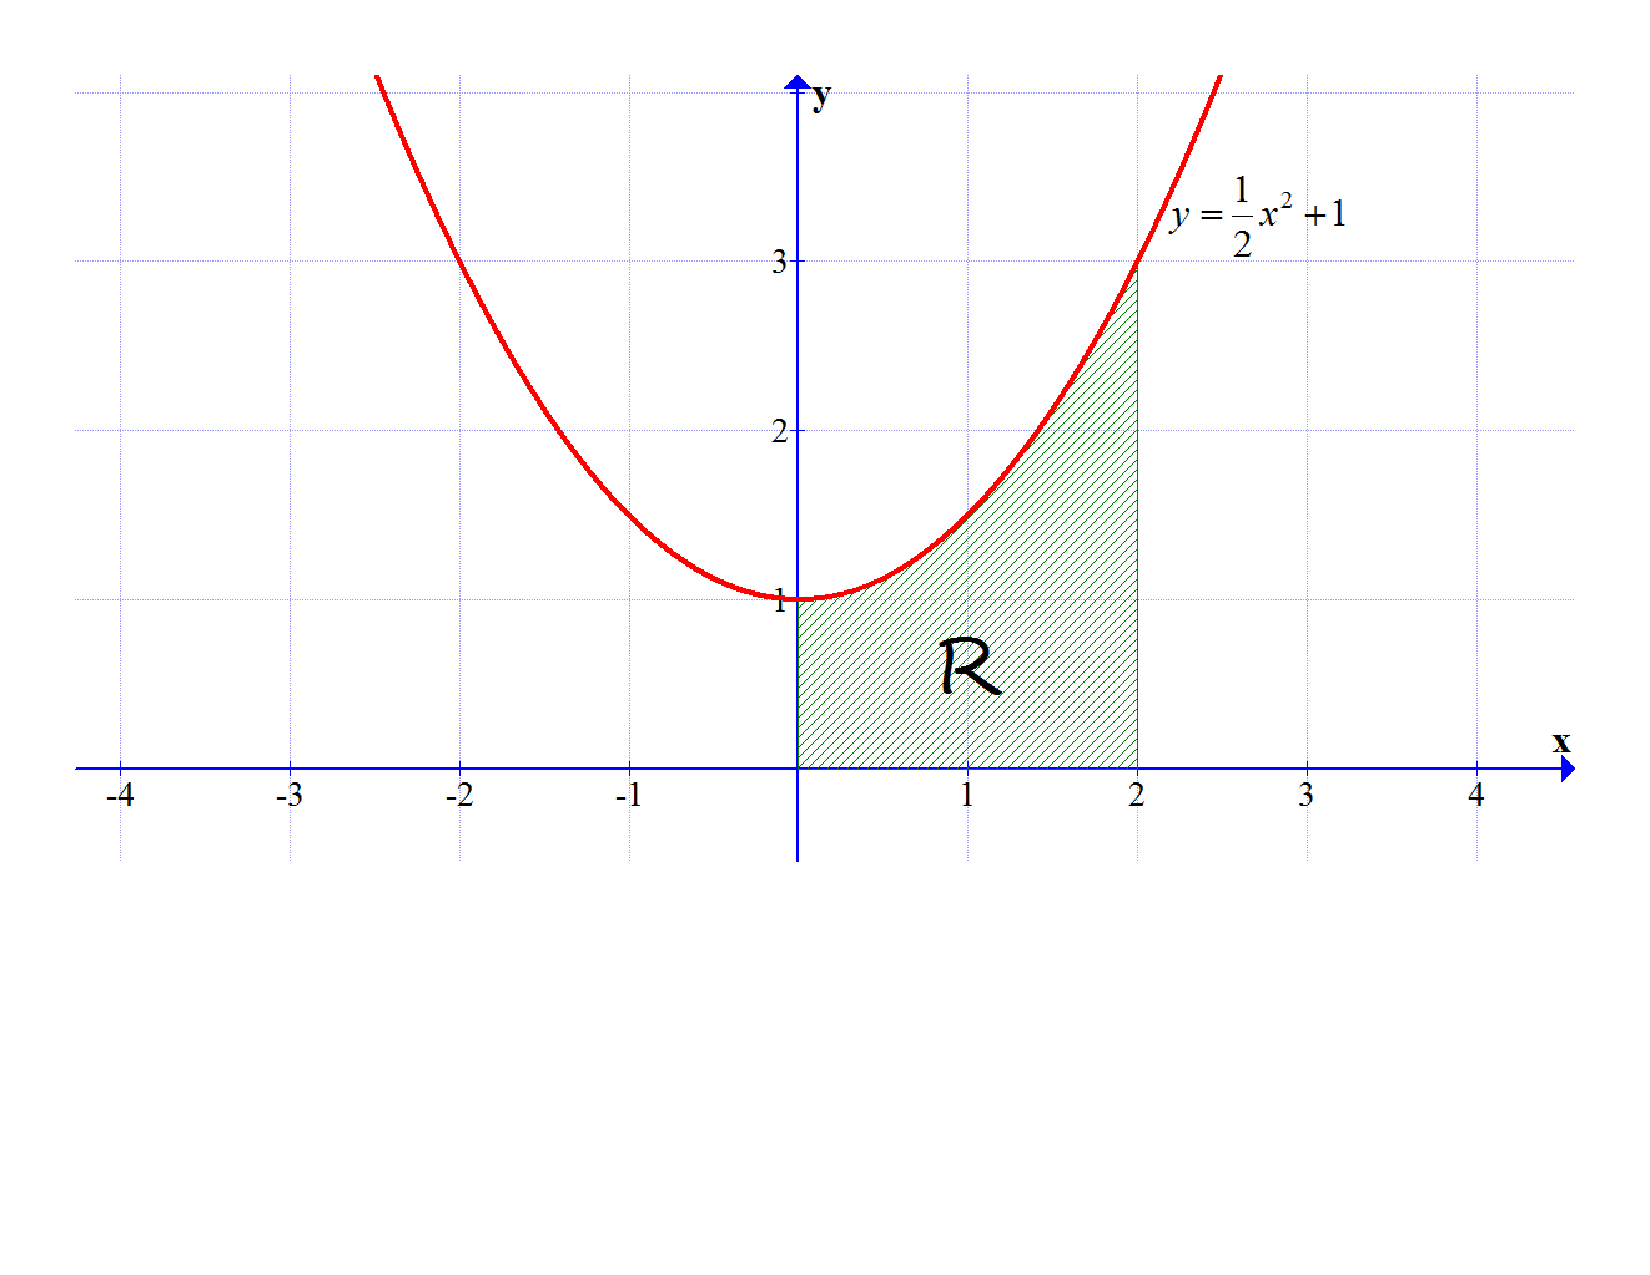
\includegraphics[scale=0.5]{graph1.pdf}

\end{center}

\includegraphics[scale=0.5]{start.pdf}
{{$\pi\int_0^2 \left(\frac{1}{2}x^2+1\right)^2 \,dx$}}
\includegraphics[scale=0.5]{end.pdf}


\newpage

\item Around the $x$-axis:

\begin{center}

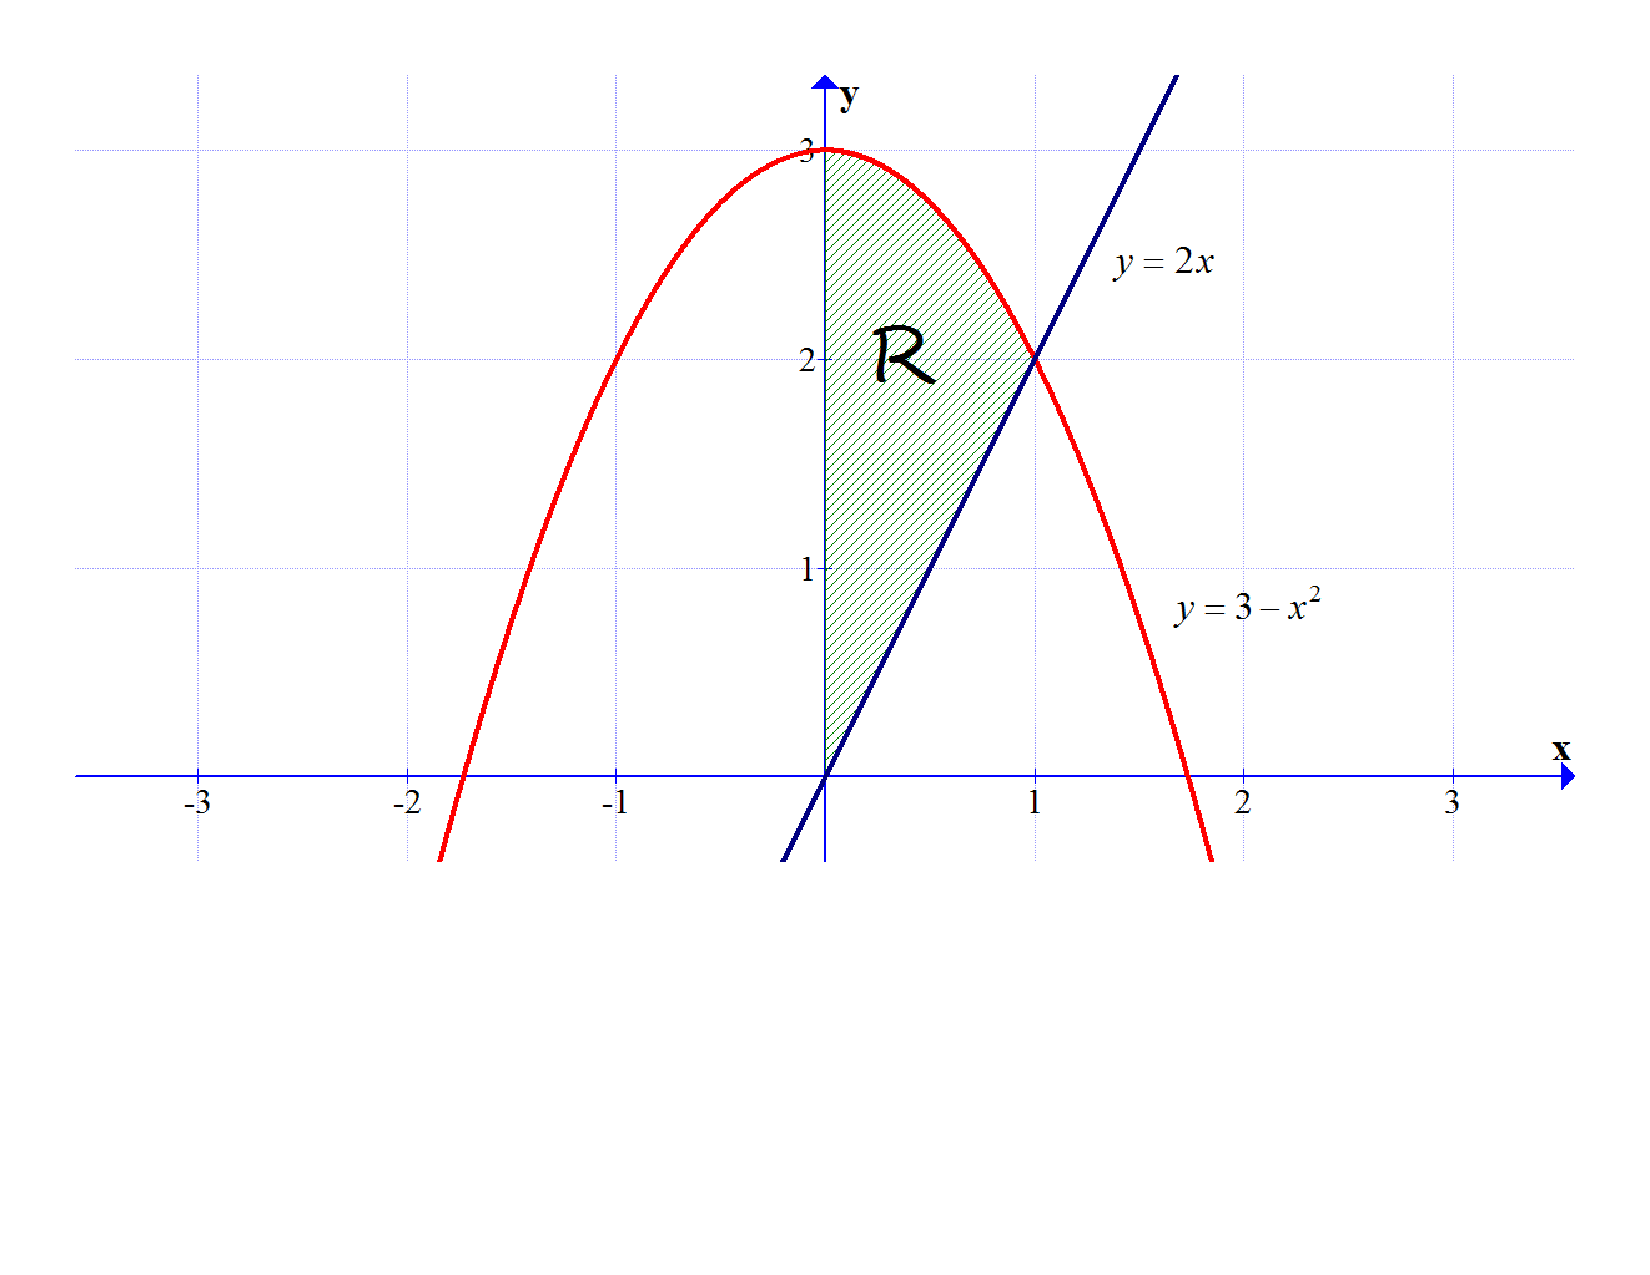
\includegraphics[scale=0.3]{graph2.pdf}

\end{center}

\includegraphics[scale=0.5]{start.pdf}
{{$\pi\int_0^1 \left((3-x^2)^2-(2x)^2\right)\,dx$}}
\includegraphics[scale=0.5]{end.pdf}


\item Around the $y$-axis:

\begin{center}

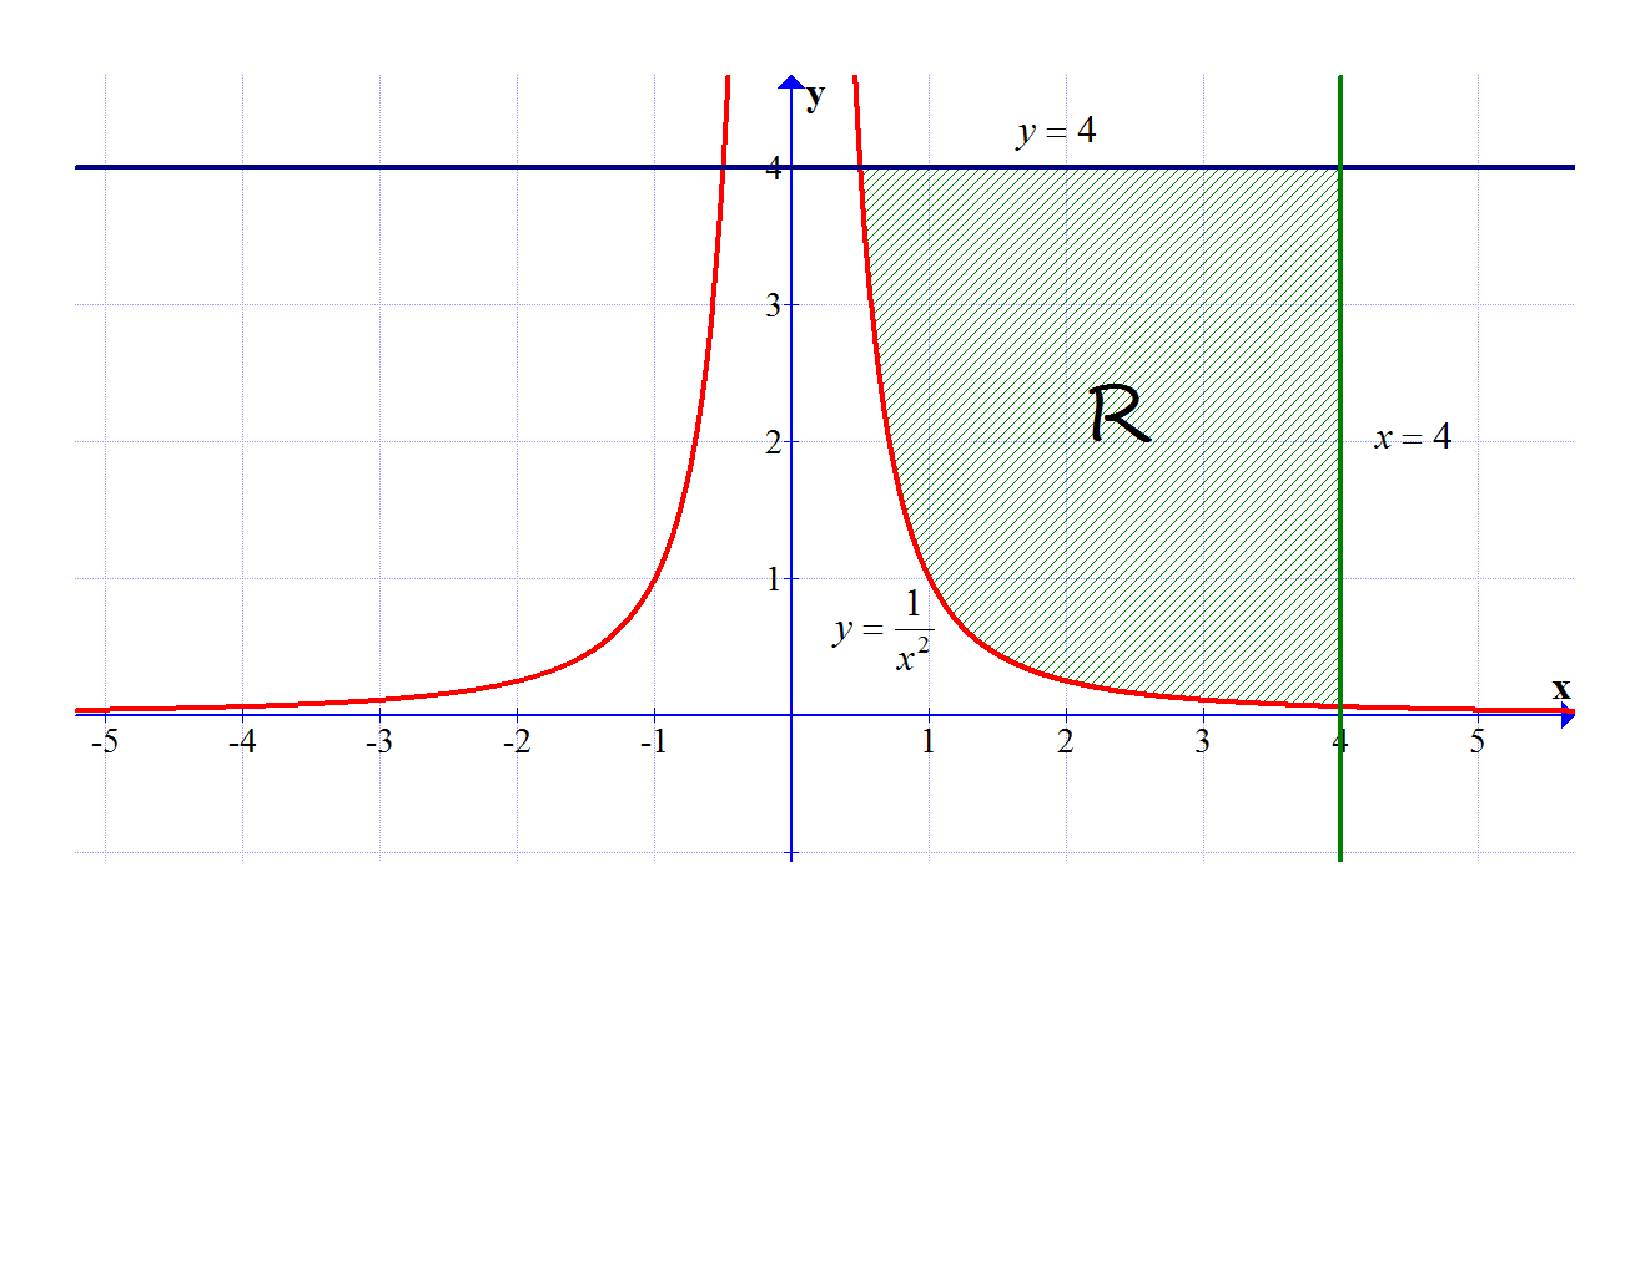
\includegraphics[scale=0.3]{graph3.pdf}

\end{center}

\includegraphics[scale=0.5]{start.pdf}
{{$\pi\int_{\frac{1}{16}}^4 \left(16-\frac{1}{y}\right) \,dy$}}
\includegraphics[scale=0.5]{end.pdf}


\item Around the $y$-axis:

\begin{center}

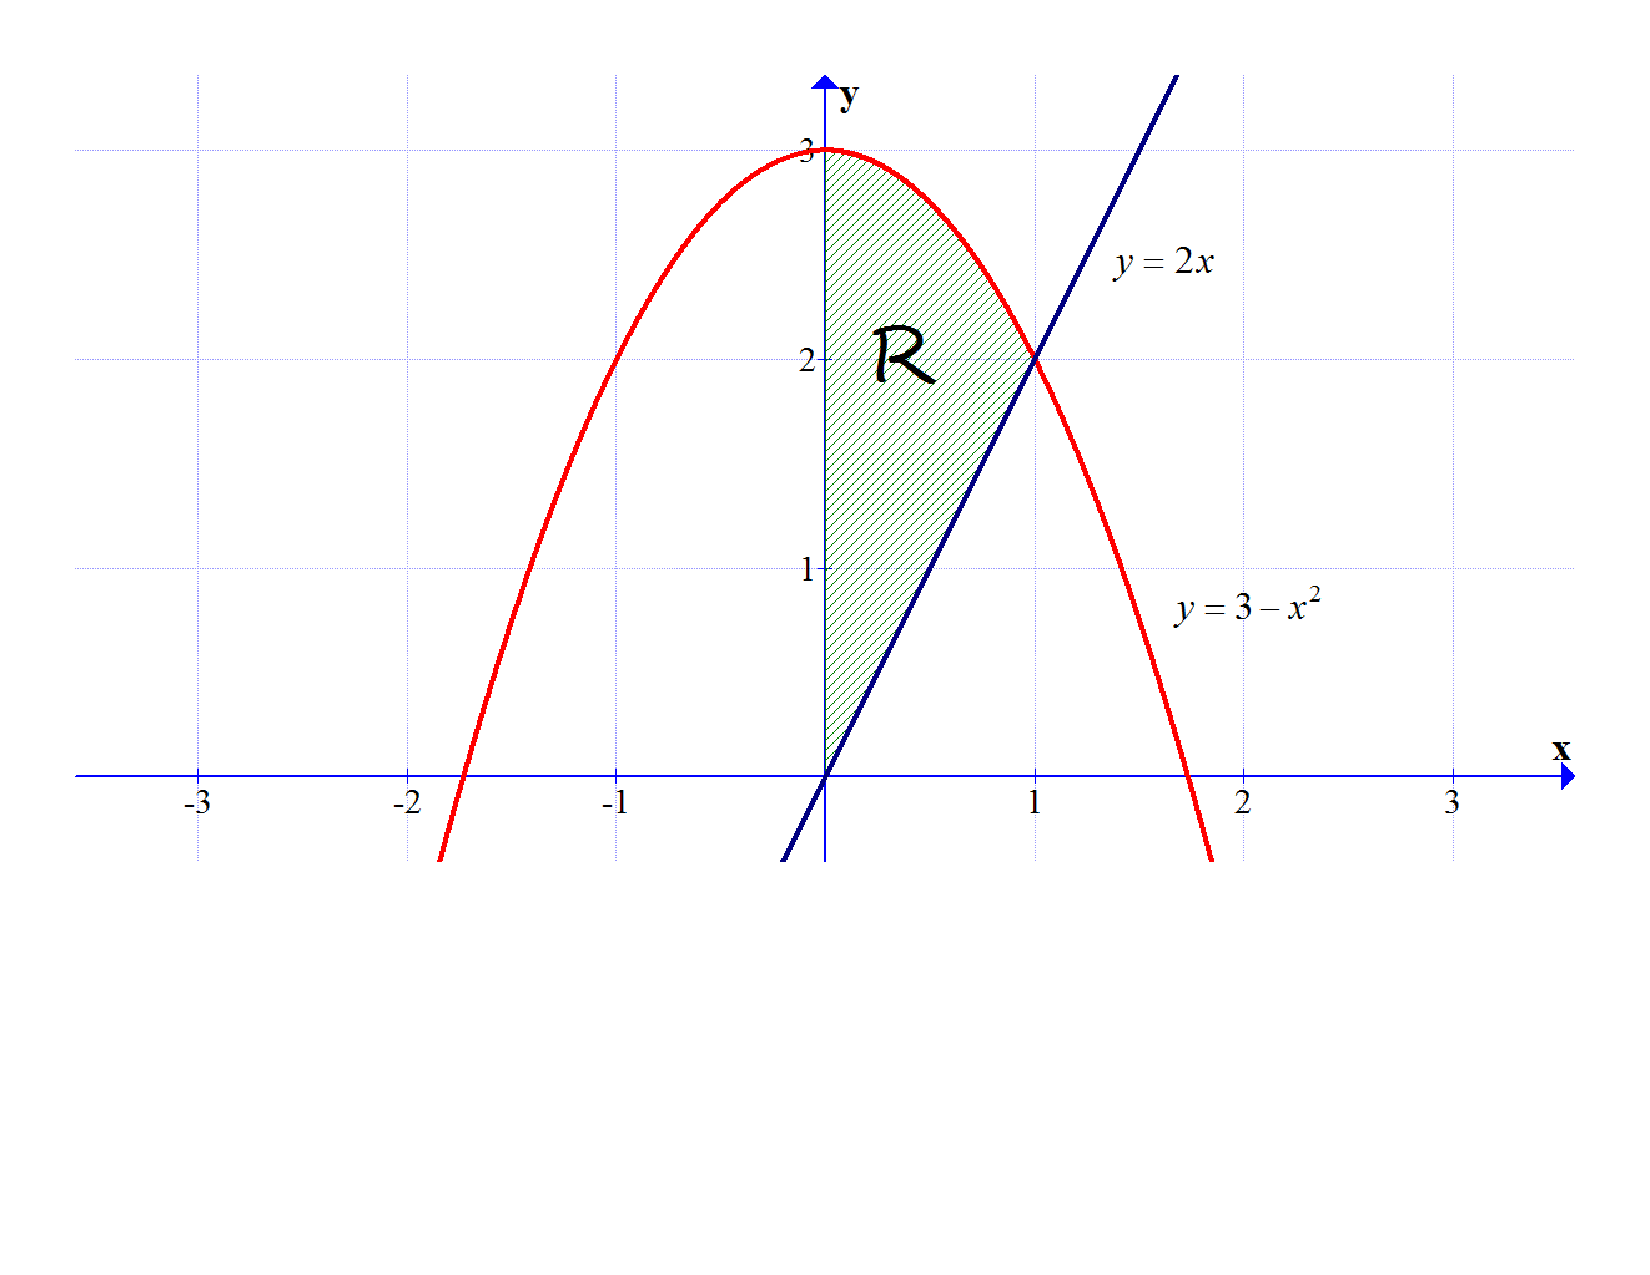
\includegraphics[scale=0.3]{graph2.pdf}

\end{center}

\includegraphics[scale=0.5]{start.pdf}
{{$\pi\int_0^2 \left(\frac{y}{2}\right)^2 \,dy+\pi\int_2^3 (3-y) \,dy$}}
\includegraphics[scale=0.5]{end.pdf}


\end{enumerate}

\end{enumerate}

\noindent{\bf For problems 2-7, compute the volume of the solid that results from revolving the region enclosed by the given curves around the $x$-axis.}

\begin{enumerate}
\setcounter{enumi}{1}

\item $y=\sqrt{4-x^2}$ and $y=0$

\includegraphics[scale=0.5]{start.pdf}
{{$\frac{32\pi}{3}$}}
\includegraphics[scale=0.5]{end.pdf}


\item $y=\sqrt{x-1}$, $x=5$, and the $x$-axis

\includegraphics[scale=0.5]{start.pdf}
{{$8\pi$}}
\includegraphics[scale=0.5]{end.pdf}


\item $y=e^x$, $y=1$, and $x=\ln{5}$

\includegraphics[scale=0.5]{start.pdf}
{{$\pi(12-\ln{5})$}}
\includegraphics[scale=0.5]{end.pdf}


\item $y=\sec{x}$, $y=\frac{1}{2}$, $x=-\frac{\pi}{4}$, and $x=\frac{\pi}{4}$

\includegraphics[scale=0.5]{start.pdf}
{{$2\pi-\frac{\pi^2}{8}$; Detailed Solution: \textcolor{blue}{\href{http://www.math.drexel.edu/classes/Calculus/resources/Math122HW/Solutions/122_08_Volume_05.pdf}{Here}}}}
\includegraphics[scale=0.5]{end.pdf}


\item $y=\sqrt{\tan{x}}$, $x=\frac{\pi}{3}$, and the $x$-axis

\includegraphics[scale=0.5]{start.pdf}
{{$\pi\ln{2}$}}
\includegraphics[scale=0.5]{end.pdf}


\item $y=\frac{1}{\sqrt{x^2+9}}$, $x=-3$, $x=3$, and the $x$ axis

\includegraphics[scale=0.5]{start.pdf}
{{$\frac{\pi^2}{6}$}}
\includegraphics[scale=0.5]{end.pdf}


\item A solid called a torus is formed by revolving the circle $x^2+(y-2)^2=1$ around the $x$-axis. 

\begin{center}
\begin{tabular}{cc}
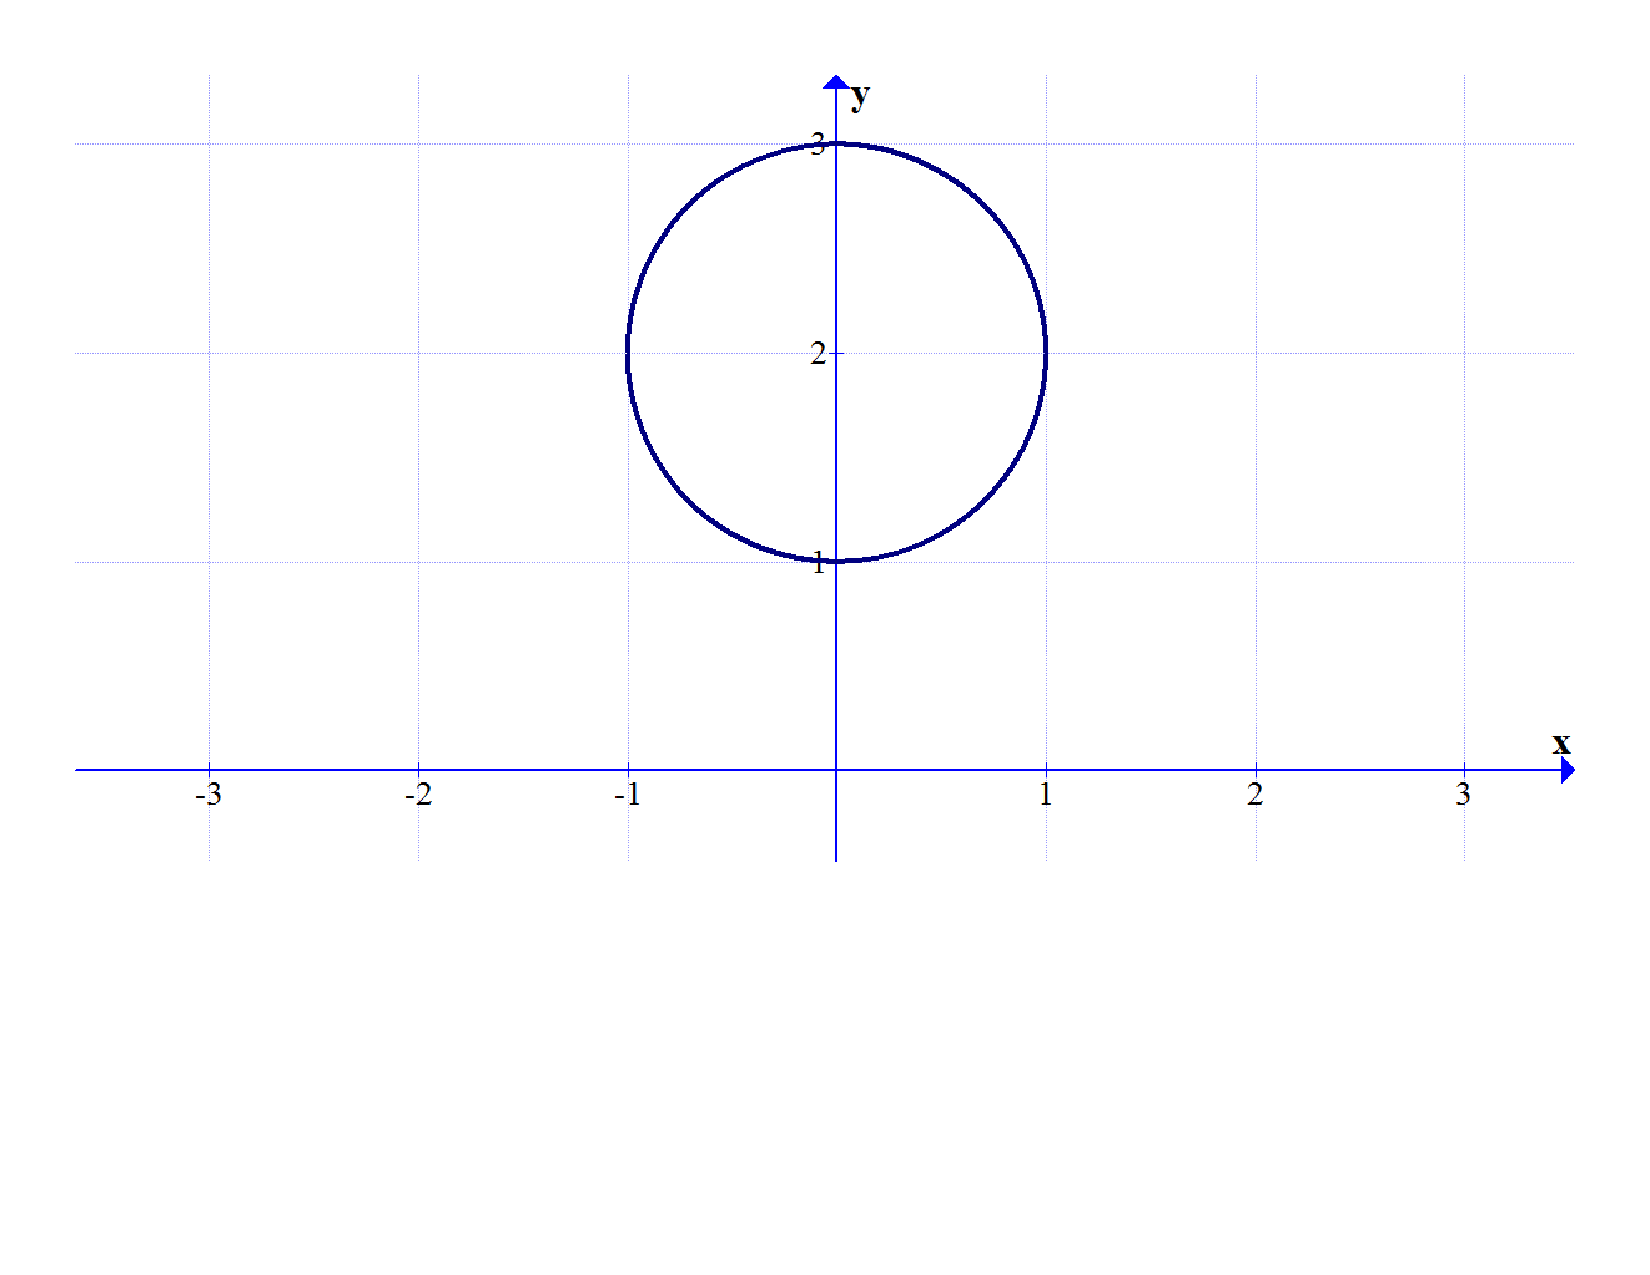
\includegraphics[scale=0.4]{circle.pdf}&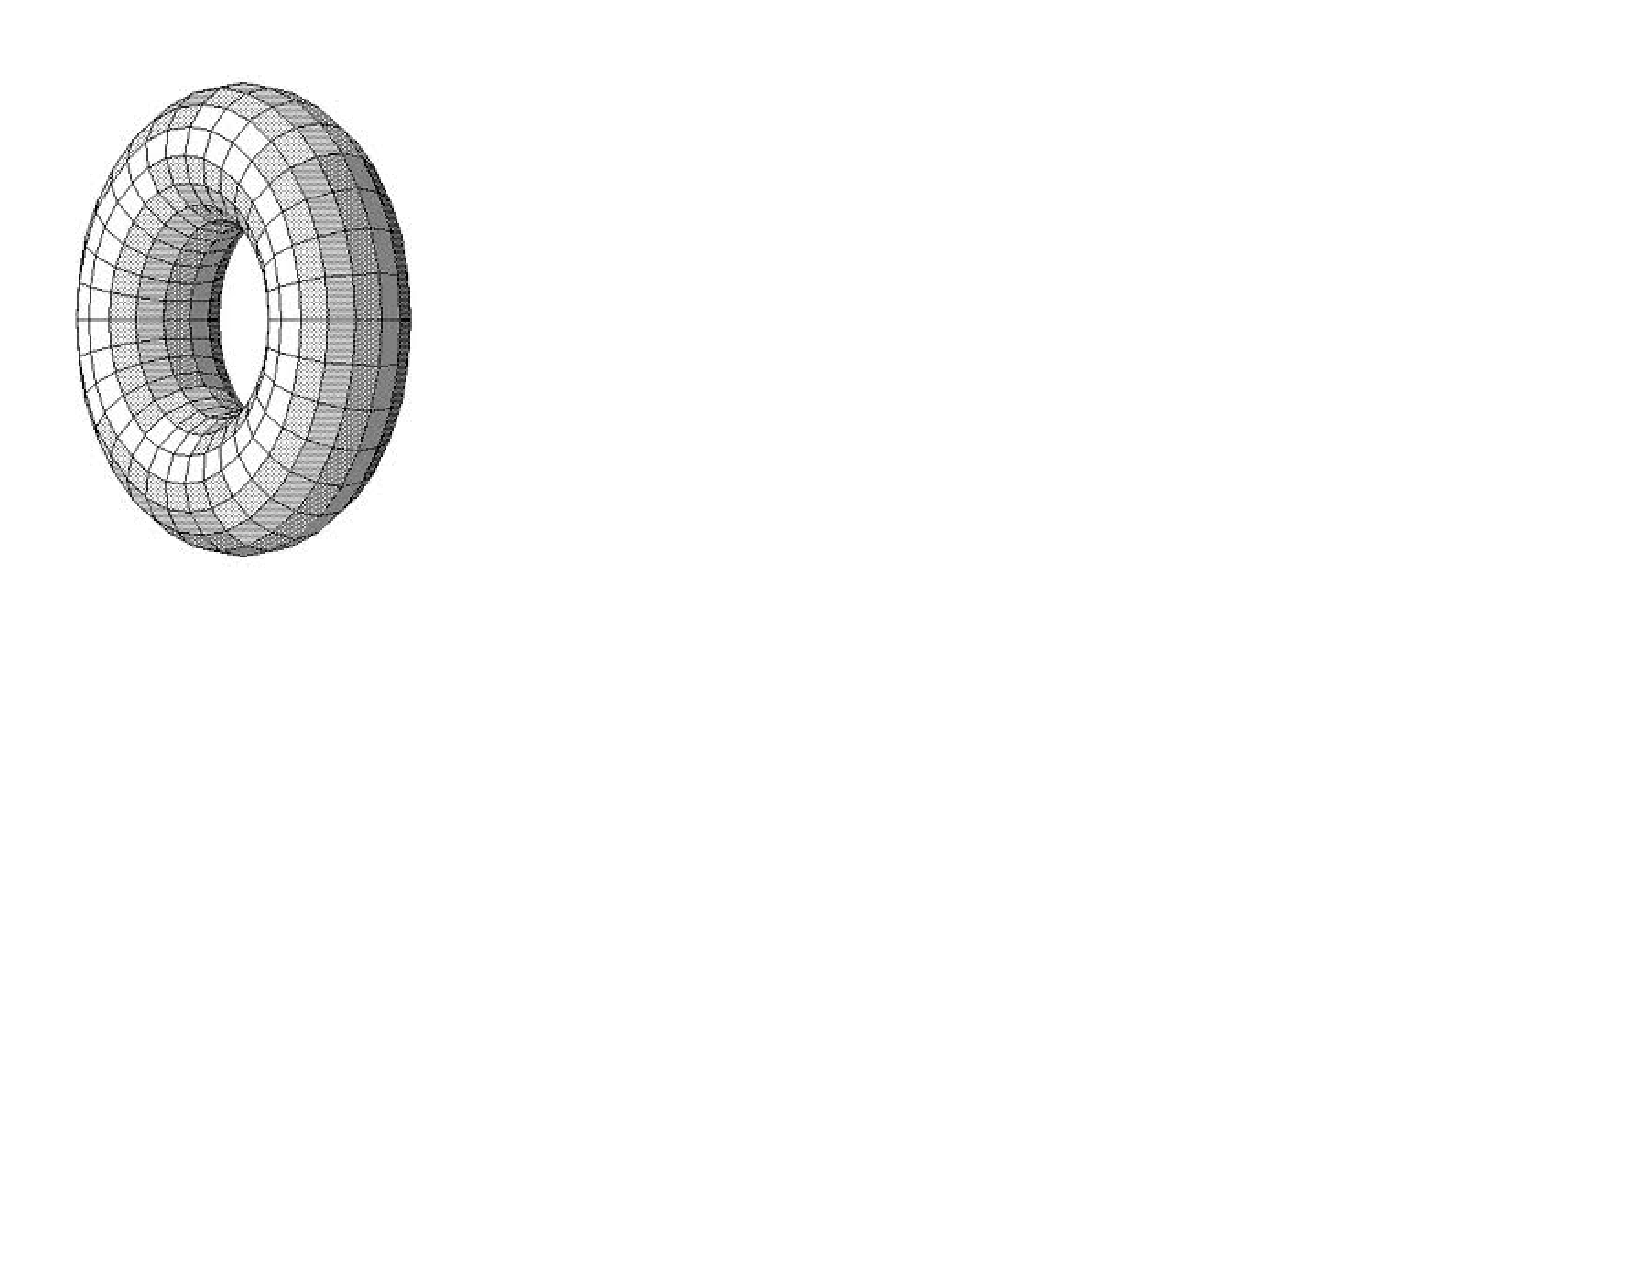
\includegraphics[scale=.7]{torus.pdf}
\end{tabular}
\end{center}

\begin{enumerate}

\item  Set up an integral which represents the volume of this solid.

\includegraphics[scale=0.5]{start.pdf}
{{$V=\pi \int_{-1}^1 \left(\left(\sqrt{1-x^2}+2\right)^2-\left(2-\sqrt{1-x^2}\right)^2\right)\,dx=8\pi\int_{-1}^1 \sqrt{1-x^2} \,dx$}}
\includegraphics[scale=0.5]{end.pdf}


\item Now, compute the volume of the torus by evaluating your integral from part (a).  {\bf Hint:} Consider using an appropriate formula from geometry at some point during your calculation.

\includegraphics[scale=0.5]{start.pdf}
{{$4\pi^2$}}
\includegraphics[scale=0.5]{end.pdf}


\end{enumerate}

\end{enumerate}

\noindent{\bf For problems 9-11, compute the volume of the solid that results from revolving the region enclosed by the given curves around the $y$-axis.}

\begin{enumerate}
\setcounter{enumi}{8}

\item $x=y^2$ and $y=2x$

\includegraphics[scale=0.5]{start.pdf}
{{$\frac{\pi}{240}$}}
\includegraphics[scale=0.5]{end.pdf}


\item $y=x^2$ and $y=2x+3$, in the first quadrant.

\includegraphics[scale=0.5]{start.pdf}
{{$\frac{45\pi}{2}$}}
\includegraphics[scale=0.5]{end.pdf}


\item $y=\ln{x}$, $x=e$, and $y=0$

\includegraphics[scale=0.5]{start.pdf}
{{$\frac{\pi}{2}\left(1+e^2\right)$; Detailed Solution: \textcolor{blue}{\href{http://www.math.drexel.edu/classes/Calculus/resources/Math122HW/Solutions/122_08_Volume_11.pdf}{Here}}}}
\includegraphics[scale=0.5]{end.pdf}


\item By revolving an appropriate region around the $x$-axis, show that the volume of a sphere with a radius of $R$ is $V=\frac{4}{3}\pi R^3$.

\begin{center}
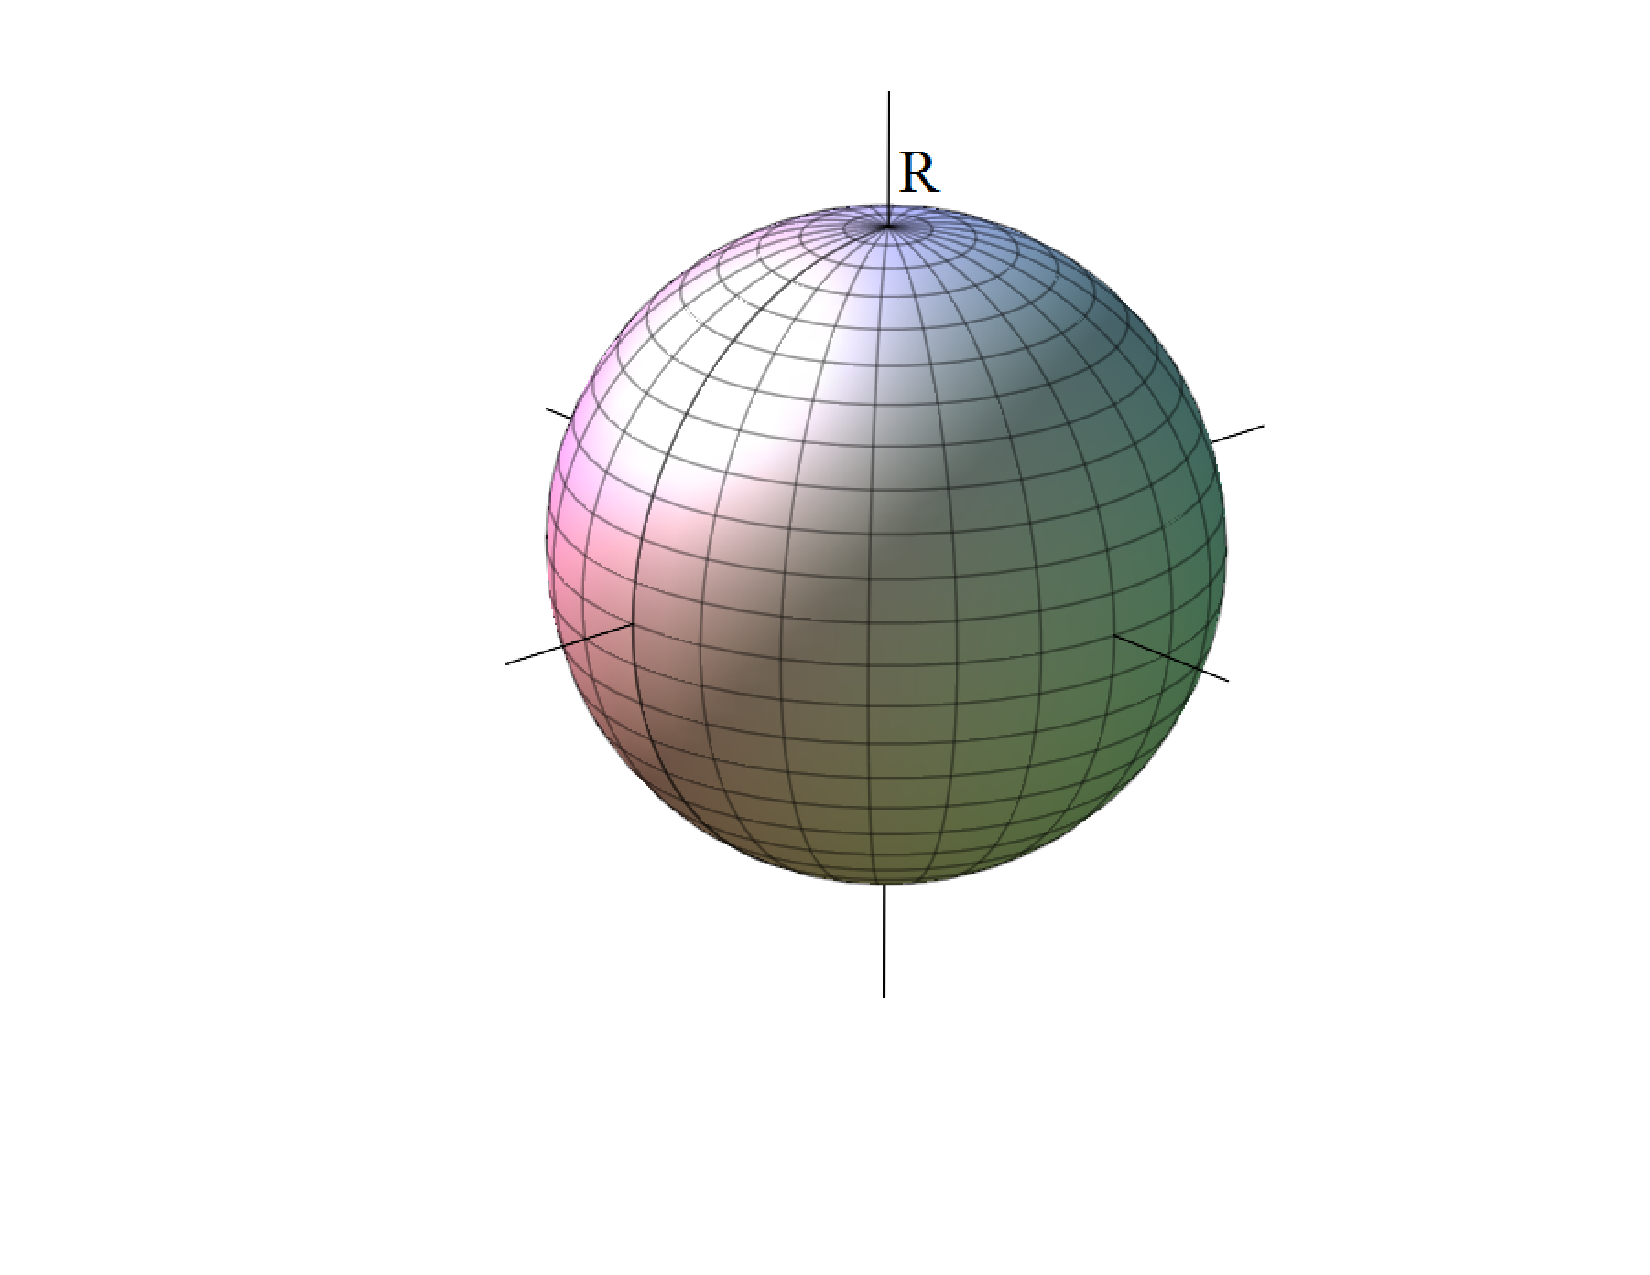
\includegraphics[scale=0.4]{sphere.pdf}
\end{center}

\includegraphics[scale=0.5]{start.pdf}
{{{1\linewidth}{We revolve the region enclosed by the semicircle $y=\sqrt{R^2-x^2}$ and the $x$ axis on the interval $[-R,R]$ around the $x$-axis.
\begin{align*}
V &= \pi \int_{-R}^R (\sqrt{R^2-x^2})^2 \,dx\\
&= \pi \int_{-R}^R (R^2-x^2) \,dx\\
&= 2\pi \int_{0}^R (R^2-x^2) \,dx\\
&=2\pi\left[R^2x-\frac{1}{3}x^3\right]_{x=0}^{x=R}\\
&=2\pi\left(R^3-\frac{R^3}{3}\right)\\
&=\frac{4\pi}{3}R^3
\end{align*}
}}}
\includegraphics[scale=0.5]{end.pdf}


\item Consider the right circular cone with a height of $h$ and a base-radius of $R$, shown below.
\begin{center}
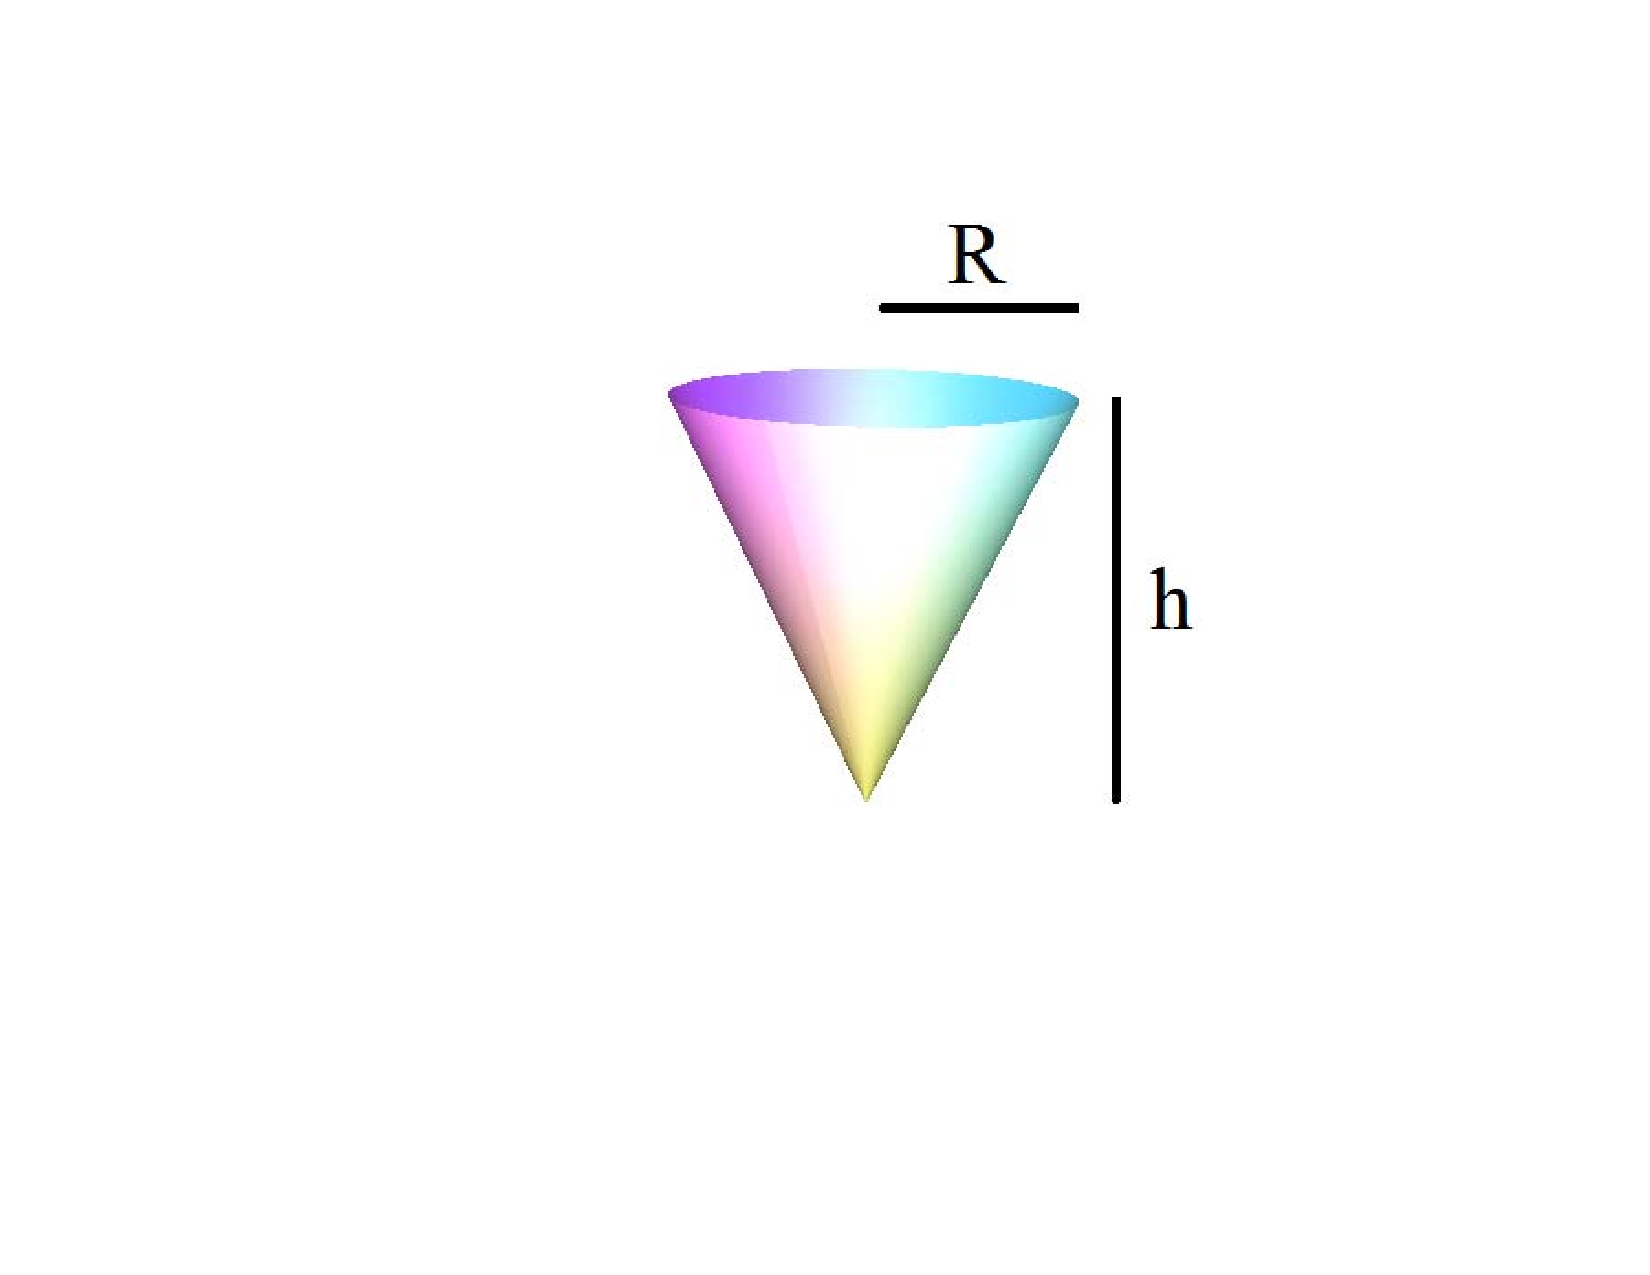
\includegraphics[scale=0.5]{cone.pdf}
\end{center}
By revolving an appropriate region around the $y$ axis, show that the volume is $V=\frac{1}{3}\pi R^2h$.

\includegraphics[scale=0.5]{start.pdf}
{{{1\linewidth}{We revolve the region enclosed by the line $y=\frac{h}{R}x$, $y=h$ and $x=0$ around the $y$-axis.
\begin{align*}
V&=\pi\int_0^h \left(\frac{R}{h}y\right)^2 \,dy\\
&=\pi\int_0^h \frac{R^2}{h^2}y^2 \,dy\\
&=\left.\frac{R^2\pi}{3h^2}y^3\right|_{y=0}^{y=h}\\
&=\frac{R^2\pi}{3h^2}h^3\\
&=\frac{1}{3}\pi R^2h
\end{align*}
}}}
\includegraphics[scale=0.5]{end.pdf}


\item Let $V$ be the volume of the solid which results from revolving the region enclosed by $y=x^3$, $x=0$, and $y=k$ $(k>0)$ around the $y$ axis.  Find the value of $k$ such that $V=9\pi$.

\includegraphics[scale=0.5]{start.pdf}
{{$k=15^{3/5}$}}
\includegraphics[scale=0.5]{end.pdf}


\item The base of a solid is the region inside of the circle $x^2+y^2=9$.  Compute the volume of the solid if all cross sections perpendicular to the $x$-axis are squares.

\includegraphics[scale=0.5]{start.pdf}
{{144}}
\includegraphics[scale=0.5]{end.pdf}


\item The base of a solid is the region enclosed by $y=\sqrt{x}$ and $y=x$.  Compute the volume of the solid if all cross sections perpendicular to the $x$-axis are semicircles.

\includegraphics[scale=0.5]{start.pdf}
{{$\frac{\pi}{240}$}}
\includegraphics[scale=0.5]{end.pdf}


\item For each of the following, compute the volume of the solid whose base is enclosed by $y=x$, $y=-x$, and $x=1$  and whose cross sections taken perpendicular to the $x$-axis are:

\begin{enumerate}

\item squares

\includegraphics[scale=0.5]{start.pdf}
{{$\frac{4}{3}$}}
\includegraphics[scale=0.5]{end.pdf}


\item semicircles

\includegraphics[scale=0.5]{start.pdf}
{{$\frac{\pi}{6}$}}
\includegraphics[scale=0.5]{end.pdf}


\item equilateral triangles

\includegraphics[scale=0.5]{start.pdf}
{{$\frac{\sqrt{3}}{3}$}}
\includegraphics[scale=0.5]{end.pdf}


\end{enumerate}

\item Let $R$ be the region enclosed by $y=x^3$, $x=2$, and $y=0$.  For each of the following, set up but do not evaluate the integral (or integrals) which represent the volume of the solid which results from revolving $R$ around the indicated line.

\begin{enumerate}

\item Revolved around $y=-1$

\includegraphics[scale=0.5]{start.pdf}
{{$\pi \int_0^2 \left((x^3+1)^2-1\right) \,dx$}}
\includegraphics[scale=0.5]{end.pdf}


\item Revolved around $y=8$

\includegraphics[scale=0.5]{start.pdf}
{{$\pi \int_0^2 \left(64-(8-x^3)^2\right) \,dx$}}
\includegraphics[scale=0.5]{end.pdf}


\item Revolved around $x=-2$

\includegraphics[scale=0.5]{start.pdf}
{{$\pi \int_0^8 \left(16-(\sqrt[3]{y}+2)^2\right)\,dy$}}
\includegraphics[scale=0.5]{end.pdf}


\item Revolved around $x=2$

\includegraphics[scale=0.5]{start.pdf}
{{$\pi \int_0^8 (2-\sqrt[3]{y})^2 \,dy$}}
\includegraphics[scale=0.5]{end.pdf}


\end{enumerate}

\item Let $R$ be the region enclosed by $y=x$ and $y=\sqrt{x}$.  For each of the following, set up but do not evaluate the integral (or integrals) which represent the volume of the solid which results from revolving $R$ around the indicated line.

\begin{enumerate}

\item Revolved around $y=1$

\includegraphics[scale=0.5]{start.pdf}
{{$\pi \int_0^1 \left((1-x)^2-(1-\sqrt{x})^2\right)\,dx$}}
\includegraphics[scale=0.5]{end.pdf}


\item Revolved around $y=-1$

\includegraphics[scale=0.5]{start.pdf}
{{$\pi \int_0^1 \left((\sqrt{x}+1)^2-(x+1)^2\right)\,dx$}}
\includegraphics[scale=0.5]{end.pdf}


\item Revolved around $x=1$

\includegraphics[scale=0.5]{start.pdf}
{{$\pi \int_0^1 \left((1-y^2)^2-(1-y)^2\right)\,dy$}}
\includegraphics[scale=0.5]{end.pdf}


\item Revolved around $x=-1$

\includegraphics[scale=0.5]{start.pdf}
{{$\pi \int_0^1 \left((1+y)^2-(1+y^2)^2\right)\,dy$}}
\includegraphics[scale=0.5]{end.pdf}


\end{enumerate}

\newpage

\item Consider the Great Pyramid of Giza, located in Egypt:

\begin{center}
\includegraphics[scale=0.45]{giza.pdf}
\end{center}

The pyramid is a triangular prism with a square base, as in the diagram below.  

\begin{center}
\includegraphics[scale=1.3]{pyramid.pdf}
\end{center}

The height of the pyramid is 138.8 meters and the base has a side length of 230.4 meters.  

\begin{enumerate} 

\item Using the fact that all cross sections taken perpendicular to the vertical height are squares, use an integral to compute the volume of the pyramid.

{\bf Hint:} Similar triangles should be useful at some point in your calculation.

\includegraphics[scale=0.5]{start.pdf}
{{$V\approx2,456,027$ square meters}}
\includegraphics[scale=0.5]{end.pdf}


\item Repeat your calculation for a triangular pyramid that has a height of $h$ and a square base of side length $b$ to derive a general formula for the volume of such a solid.

\includegraphics[scale=0.5]{start.pdf}
{{$V=\int_0^h \left(\frac{b}{h}z\right)^2 \,dz=\frac{1}{3}b^2h$}}
\includegraphics[scale=0.5]{end.pdf}


\end{enumerate}

\end{enumerate}

\end{document}